\documentclass[10pt,t,aspectratio=169]{beamer}
%\usetheme{Berkeley}
\usepackage{graphicx}
\usepackage{amsmath}
\usepackage[american]{circuitikz}

% Packages to plot functions
\usepackage{pgfplots}
\pgfplotsset{compat=newest}

\usepackage{multicol}
\usepackage{multirow}
\usepackage{textcomp} % to use \textmu
\usepackage[absolute,overlay]{textpos} % to place floating text boxes with \begin{textblock*}{width}(x,y)
\usepackage{tcolorbox}
\usepackage{colortbl} % allows coloring cells of a table with \cellcolor{blue!25}

\title{Clase 4}
\subtitle{Arrastre y difusión}
\author{Dr.-Ing. Juan José Montero Rodríguez}
\subject{Elementos Activos}
\institute{Escuela de Ingeniería Electrónica}
\date{Semestre II-2023}
\titlegraphic{\includegraphics[height=12mm]{figures/logoTEC.pdf}}


\begin{document}

\begin{frame}[t]
\titlepage
\end{frame}


\begin{frame}[t]
    \frametitle{Transporte de Portadores de Carga}

    La corriente eléctrica consiste en el movimiento de cargas: electrones y huecos.

    \vspace{3mm}
    Los átomos de dopado pueden ionizarse como parte del proceso de conducción eléctrica:

    \begin{itemize}
        \item Los átomos donadores se ionizan positivamente al ceder un electrón para la conducción eléctrica ($N_D^+$).
        \item Los átomos aceptores se ionizan negativamente al recibir un electrón durante la conducción eléctrica ($N_A^-$).
        \item En semiconductores, los dopantes ionizados son inmóviles y no contribuyen a la conducción.
        
    \end{itemize}

    \vspace{3mm}
    Existen dos mecanismos de transporte de portadores de carga

    \begin{itemize}
        \item Corriente de \textbf{arrastre}, debido a la aplicación de un campo eléctrico.
        \item Corriente de \textbf{difusión}, debido a gradientes de concentración de portadores de carga.
    \end{itemize}
\end{frame}


\begin{frame}[t]
    \frametitle{Arrastre (Drift)}

    \begin{multicols}{2}
        1. En un semiconductor sin campo E, los electrones se mueven de manera aleatoria (movimiento browniano). El flujo neto es cero.

        \[ I = 0 \]

        2. Una partícula cargada experimenta una fuerza al ser sometida a un campo eléctrico externo.

        \[ F = m\cdot{}a \]

        3. Un electrón aislado en presencia de campo eléctrico experimenta aceleración constante: velocidad aumenta.

        \[ F = -qE = m\cdot{}\dfrac{dv}{dt} \]

        4. Dentro de un material, la velocidad que se genera no es la misma por colisiones y fuerzas en el cristal. 

        \[ v_d = \mu{}\cdot{}E \]

        5. La constante $\mu_n$ es la movilidad de los electrones dentro del cristal.

        \[ \mu_n = 1350\ cm^2/Vs \]

        6. Lo mismo ocurre con los huecos dentro del cristal, aunque la movilidad $\mu_p$ es menor que la de los electrones

        \[ \mu_p = 480\ cm^2/Vs \]
    \end{multicols}
\end{frame}


\begin{frame}[t]
    \frametitle{Corriente de Arrastre}

    \begin{itemize}
        \item De acuerdo con la Ley de Ohm, la corriente fluye al aplicar un campo eléctrico externo.
    \end{itemize}
    
    \begin{columns}
        \begin{column}{0.5\textwidth}
            \centering
            \includegraphics[width=0.5\textwidth]{./figures/drift1.png}
            %
            \[ J_{drift} = \sigma E \]
            %
            \[ \sigma = (qn\mu_n + qp\mu_p) \]
            %
            \[ J_{drift} = (qn\mu_n + qp\mu_p)E \]
        \end{column}
        \begin{column}{0.5\textwidth}
            \centering
            \includegraphics[width=0.7\textwidth]{./figures/drift2.png}

            \begin{itemize}
                \item J: densidad de corriente de arrastre
                \item $\sigma$: conductividad
                \item E: campo eléctrico
                \item q: carga del electrón
                \item n: concentración de portador de carga
                \item $\mu$: movilidad del portador de carga

            \end{itemize}
        
        \end{column}
    \end{columns}

\end{frame}


\begin{frame}[t]
    \frametitle{Movilidad y Velocidad de Arrastre}

    \begin{itemize}
        \item En ausencia de un campo eléctrico, el electrón presenta un movimiento térmico aleatorio con una velocidad térmica promedio $v_t$.
        \item Al aplicar un campo eléctrico, el electrón adquiere una velocidad de arrastre determinada por:
    \end{itemize}
    
    \begin{columns}
    
        \begin{column}{0.5\textwidth}
        
            \[ v_d = \mu{}\cdot{}E \]
            
        \end{column}
        
        \begin{column}{0.5\textwidth}
        
            $v_d$: velocidad de arrastre (cm/s)
            
            $\mu$: movilidad ($cm^2/Vs$)
            
            $E$: campo eléctrico (V/cm)
            
        \end{column}

        
    \end{columns}
    %
    \vspace{5mm}
    \begin{itemize}
        \item Para $E>10^5\ V/cm$ la velocidad de arrastre se satura $\approx{}10^7\ cm/s$
        \item Los electrones tienen una movilidad mayor que los huecos en un factor de 2..3 $\rightarrow$ ante un campo eléctrico, los electrones son 2..3 veces más rápidos que los huecos.
        \item La movilidad está determinada por: masa efectiva, dispersión por impurezas, dispersión por la estructura cristalina.
    \end{itemize}
\end{frame}


\begin{frame}[t]
    \frametitle{Saturación de la Velocidad de Arrastre}

    \begin{columns}
    
        \begin{column}{0.5\textwidth}
        
            La velocidad de arrastre no puede aumentar de manera indefinida. 
            
            \begin{itemize}
                \item Colisiones entre los electrones contra los átomos de la red del cristal.
                \item Fuerzas de atracción/repulsión entre electrón-electrón.
            \end{itemize}
            %
            Este efecto se modela por medio de la siguiente ecuación:
            %
            \[ \mu = \dfrac{\mu_0}{1+bE} \]
            %
            Donde $\mu_0$ es la movilidad en ausencia de campo eléctrico, $E$ es el campo eléctrico aplicado y $b=\mu_0/v_{sat}$
            
        \end{column}
        
        \begin{column}{0.5\textwidth}
        
            \centering
            \includegraphics[width=6cm]{./figures/vdsat.png}

            \flushleft
            La velocidad de saturación $v_{sat}$ es una constante determinada de forma experimental. Esto permite reescribir la velocidad de arrastre como:

            \[ v_d = \dfrac{\mu_0}{1+\dfrac{\mu_0E}{v_{sat}}}\times{}E \]

        \end{column}
        
    \end{columns}
    
\end{frame}


\begin{frame}[t]
    \frametitle{Ejemplo: Saturación de la Velocidad de Arrastre}

    Un bloque de silicio con longitud $L=0.2\ \mu{}m$, tiene una tensión de 1 V entre sus extremos. Considere $\mu_n=1350\ cm^2/Vs$ y $v_{sat}=10^7\ cm/s$.

    \begin{columns}
    
        \begin{column}{0.5\textwidth}
        
            \begin{itemize}
                \item Determine la movilidad efectiva bajo estas condiciones.
            \end{itemize}
            
            \[ E = \dfrac{V}{L} = \dfrac{1\ V}{0.2\ \mu{}m} = 50\ kV/cm \]
            %
            \[ \mu = \dfrac{\mu_0}{1 + \dfrac{\mu_0E}{v_{sat}}} = \dfrac{1350}{1 + \dfrac{(1350)(50\times{}10^3)}{(10^7)}} \]
            %
            \[ \mu = \dfrac{1350}{7.75} = 174\ cm^2/Vs \]
            
        \end{column}
        
        \begin{column}{0.5\textwidth}
        
            \begin{itemize}
                \item Calcule la tensión máxima permitida de modo que la movilidad efectiva no sea reducida más de un 10\%.
            \end{itemize}
            
            \[ 0.9\mu_0 = \dfrac{\mu_0}{1 + \dfrac{\mu_0E}{v_{sat}}} \]
            %
            \[ E = \dfrac{1}{9}\dfrac{v_{sat}}{\mu_0} = 823\ V/cm \]
            %
            \[ V = E \times{} L \]
            %
            \[ V = (823\ V/cm) \times{} (0.2\times{}10^{-4}\ cm) \]
            %
            \[ V = 16.5\ mV \]
            
        \end{column}
        
    \end{columns}
    
\end{frame}


\begin{frame}[t]
    \frametitle{Movilidad en Función de la Concentración de Dopado}

    \begin{columns}
        \begin{column}{0.5\textwidth}
            El efecto del dopado en la movilidad se modela por medio de la ecuación:

            \[ \mu = \mu_{min} + \dfrac{\mu_0}{1 + \left( \dfrac{N}{N_{ref}} \right)^\alpha} \]

            Donde $N$ es la concentración total de dopantes:
            
            \[N = N_D + N_A\]

            \vspace{3mm}
            \centering
            \textbf{Valores de referencia}

            \begin{columns}
            
                \begin{column}{0.5\textwidth}
                
                    Para electrones:

                    \vspace{2mm}
                    Nref = 1.3e17 cm\textsuperscript{-3}

                    umin = 92 cm\textsuperscript{2}/Vs
                    
                    u0 = 1268 cm\textsuperscript{2}/Vs
                    
                    alpha = 0.91
                    
                \end{column}
                
                \begin{column}{0.5\textwidth}
                
                    Para huecos:

                    \vspace{2mm}
                    Nref = 2.3e17 cm\textsuperscript{-3}

                    umin = 54 cm\textsuperscript{2}/Vs
                    
                    u0 = 407 cm\textsuperscript{2}/Vs
                    
                    alpha = 0.88
                    
                \end{column}
                
            \end{columns}
            
        \end{column}
        
        \begin{column}{0.5\textwidth}
        
            \centering
            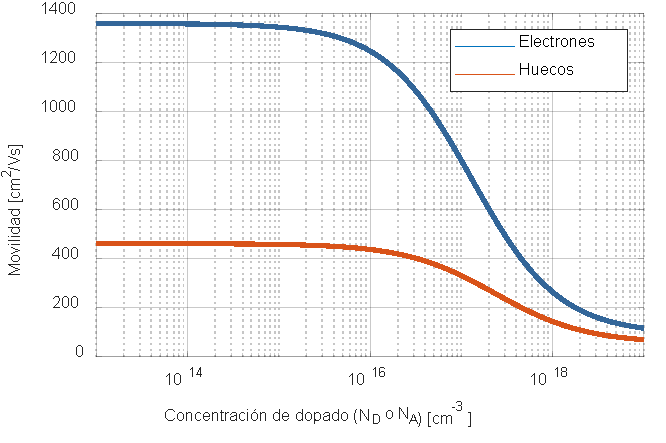
\includegraphics[width=\textwidth]{./figures/movilidad-vs-dopado.pdf}
            
        \end{column}
        
    \end{columns}
    
\end{frame}


\begin{frame}[t]
    \frametitle{Movilidad en Función de la Temperatura}

    \centering
    \includegraphics[width=5.6cm]{./figures/movilidad-vs-T-1.jpg}
    \includegraphics[width=5.6cm]{./figures/movilidad-vs-T-2.jpg}
\end{frame}


\begin{frame}[t]
    \frametitle{Resistividad}

    \begin{columns}
    
        \begin{column}{0.5\textwidth}
        
            La resistividad ($\rho$) mide la oposición inherente del material al flujo de corriente. Es el inverso de la conductividad ($sigma$).
            %
            \begin{itemize}
                \item No depende de las dimensiones físicas del material.
            \end{itemize}
            %
            \[ \mathcal{E} = \rho \cdot J \]
            %
            Se calcula como:
            %
            \[ \rho = \dfrac{1}{q(\mu_n n + \mu_p p)} \]
            %
            \begin{columns}
            
                \begin{column}{0.5\textwidth}
                
                    En semiconductores N:
                    %
                  \[ \rho \approx \dfrac{1}{q\mu_n n} \]
                  
                \end{column}
                
                \begin{column}{0.5\textwidth}
                
                    En semiconductores P:
                    %
                   \[ \rho \approx \dfrac{1}{q\mu_p p} \]
                   
                \end{column}
                
            \end{columns}
            
        \end{column}
        
        \begin{column}{0.5\textwidth}
        
            \centering
            \includegraphics[height=7cm]{./figures/resistividad.png}
            
        \end{column}
        
    \end{columns}
    
\end{frame}


\begin{frame}[t]
    \frametitle{Difusión (Diffusion)}

    \begin{columns}
    
        \begin{column}{0.5\textwidth}
        
            \begin{itemize}
                \item Si una gota de tinta cae en un vaso de agua, después de unas horas la concentración de tinta es uniforme en todo el vaso, aunque la concentración inicial estuviera localizada en un único punto.
                \item Las moléculas de tinta ``fluyen'' de una mayor concentración a una menor concentración. No son partículas cargadas: el movimiento térmico aleatorio las mueve y distribuye de manera uniforme.
                \item Lo mismo sucede con los electrones y los huecos: avanzan de mayor a menor concentración debido al movimiento térmico.
            \end{itemize}
            
        \end{column}
        
        \begin{column}{0.5\textwidth}
        
            \centering
            \includegraphics[height=7cm]{./figures/difusion.pdf}
            
        \end{column}
        
    \end{columns}
    
\end{frame}


\begin{frame}[t]
    \frametitle{Difusión (Diffusion)}

    Obedece a la ley de Fick:	

    \[ F = -D \nabla \eta \]

    \begin{itemize}
        \item D: Coeficiente de difusión, medido en cm\textsuperscript{2}/s
        \item $\eta$: Concentración de las partículas que se difunden
        \item $\nabla{}\eta$: Gradiente de concentración
    \end{itemize}

    \vspace{5mm}
    El flujo de partículas es proporcional al gradiente de concentración.

    \vspace{3mm}
    Un gradiente apunta en la dirección de menor a mayor concentración.

    \vspace{3mm}
    El gradiente en tres dimensiones:

    \[ \nabla{}\eta = \dfrac{\partial{}\eta}{\partial{}x} \hat{x} + \dfrac{\partial{}\eta}{\partial{}y} \hat{y} + \dfrac{\partial{}\eta}{\partial{}z} \hat{z} \]
\end{frame}


\begin{frame}[t]
    \frametitle{Corriente de Difusión}

    \begin{columns}
    
        \begin{column}{0.5\textwidth}
        
            Para semiconductores:
            %
            \[ J_{dif,n} = q\cdot{}D_n\cdot{}\nabla{}n \]
            %
            \[ J_{dif,p} = q\cdot{}D_p\cdot{}\nabla{}p \]

            En una dimensión:
            %
            \[ J_{dif,n} = q\cdot{}D_n\cdot{}\dfrac{dn}{dx} \hat{x} \]
            %
            \[ J_{dif,p} = q\cdot{}D_p\cdot{}\dfrac{dp}{dx} \hat{x} \]

            El coeficiente de difusión es:
            %
            \[ D_n = 34\ cm^2/s \]
            %
            \[ D_p = 12\ cm^2/s \]
            
        \end{column}
        
        \begin{column}{0.5\textwidth}
        
            \centering
            \includegraphics[width=7cm]{./figures/difusion-ej-1.png}

            \vspace{5mm}
            \includegraphics[width=5cm]{./figures/difusion-ej-2.png}
            
        \end{column}
        
    \end{columns}
    
\end{frame}


\begin{frame}[t]
    \frametitle{Experimento de Punta Caliente (Hot Probe)}

    Permite determinar si una oblea es de tipo P o de tipo N.

    \begin{figure}[H]
        \centering
        \includegraphics[width=10cm]{./figures/hotprobe.png}
    \end{figure}

    \begin{itemize}
        \item Si la oblea es tipo P, al tocar con la punta caliente, los huecos se difunden alejándose, produciendo una región ligeramente negativa.
        \item Si la oblea es tipo N, al tocar con la punta caliente, los electrones se difunden alejándose, produciendo una región ligeramente positiva.
        \item El galvanómetro permite detectar estas corrientes con direcciones opuestas.
    \end{itemize}
\end{frame}


\begin{frame}[t]
    \frametitle{Relación de Einstein}

    Relaciona la movilidad con el coeficiente de difusión:

    \[ D = V_t \cdot{} \mu \]

    \[ V_t = \dfrac{kT}{q} \approx 26\ mV @ 300\ K \]

    \centering
    \includegraphics[width=10cm]{./figures/driftanddiff.png}
\end{frame}


\begin{frame}[t]
    \frametitle{Ejemplo: Arrastre}

    Una barra de silicio tiene dimensiones 10 \textmu{}m x 5 \textmu{}m x 4 \textmu{}m.  La barra está dopada de manera uniforme, con una concentración de huecos 10\textsuperscript{15} cm\textsuperscript{-3}. Se aplica una tensión de 1 V entre las terminales, según se ilustra en la figura. Para estas condiciones, calcule:

    \begin{enumerate}
        \item La concentración de portadores de carga minoritarios.
        \item La densidad de corriente $J_{drift}$ y la corriente total en la barra.
        \item La velocidad de arrastre $v_d$ de electrones y huecos.
    \end{enumerate}

    \centering
    \includegraphics[width=6cm]{./figures/ejemplo-arrastre.png}
\end{frame}

\begin{frame}[t]
    \frametitle{Ejemplo: Difusión}

    Se inyectan huecos de manera constante en una región de silicio tipo N. En estado estable, se establece el perfil de concentración de huecos mostrado en la figura. Encuentre:

    \begin{enumerate}
        \item La magnitud, dirección y unidades del gradiente de concentración $\nabla{p}$
        \item La densidad de corriente de difusión $J_{diff}$
    \end{enumerate}

    \centering
    \includegraphics[width=6cm]{./figures/ejemplo-difusion.png}
\end{frame}


\begin{frame}{Lecturas recomendadas}
    
\end{frame}

\end{document}
